\documentclass[tikz,border=4pt]{standalone}
\usepackage{amsmath}
\begin{document}
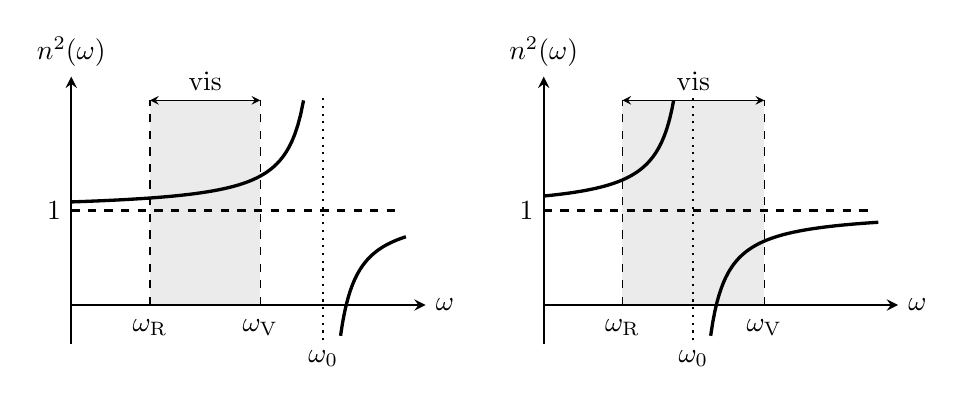
\begin{tikzpicture}[>=stealth, thick, scale=1.0]
  % Left: Quartz (omega_0 > omega_V, ultraviolet)
  \begin{scope}[xshift=0cm]
    \fill[black!8] (1.0, 0) rectangle (2.4, 2.6);
    \draw[->] (0, 0) -- (4.5, 0) node[right] {$\omega$};
    \draw[->] (0, -0.5) -- (0, 2.9) node[above] {$n^2(\omega)$};
    \draw[dashed] (0, 1.2) -- (4.2, 1.2);
    \node[left] at (0, 1.2) {$1$};

    \draw[dashed, thin] (1.0, 0) -- (1.0, 2.6);
    \draw[dashed, thin] (2.4, 0) -- (2.4, 2.6);
    \draw[<->, thin] (1.0, 2.6) -- (2.4, 2.6) node[midway, above] {$\mathrm{vis}$};
    \node[below] at (1.0, -0.05) {$\omega_{\mathrm{R}}$};
    \node[below] at (2.4, -0.05) {$\omega_{\mathrm{V}}$};

    % Asymptote omega_0 = 3.2
    \draw[dotted, thick] (3.2, -0.45) -- (3.2, 2.65);
    \node[below] at (3.2, -0.45) {$\omega_0$};

    % n^2 = 1.2 + 0.55 / (3.2^2 - x^2) * 3.0 -> adjust to stay in [-0.4, 2.6]
    % Use 1.2 + 0.35 / (3.2 - x) for clean visual shape
    \draw[very thick, domain=0:2.95, samples=80] plot (\x, {1.2 + 0.35 / (3.2 - \x)});
    \draw[very thick, domain=3.42:4.25, samples=60] plot (\x, {1.2 - 0.35 / (\x - 3.2)});
  \end{scope}

  % Right: Substance F (omega_0 inside visible band, green)
  \begin{scope}[xshift=6.0cm]
    \fill[black!8] (1.0, 0) rectangle (2.8, 2.6);
    \draw[->] (0, 0) -- (4.5, 0) node[right] {$\omega$};
    \draw[->] (0, -0.5) -- (0, 2.9) node[above] {$n^2(\omega)$};
    \draw[dashed] (0, 1.2) -- (4.2, 1.2);
    \node[left] at (0, 1.2) {$1$};

    \draw[dashed, thin] (1.0, 0) -- (1.0, 2.6);
    \draw[dashed, thin] (2.8, 0) -- (2.8, 2.6);
    \draw[<->, thin] (1.0, 2.6) -- (2.8, 2.6) node[midway, above] {$\mathrm{vis}$};
    \node[below] at (1.0, -0.05) {$\omega_{\mathrm{R}}$};
    \node[below] at (2.8, -0.05) {$\omega_{\mathrm{V}}$};

    % Asymptote omega_0 = 1.9 (middle of visible band)
    \draw[dotted, thick] (1.9, -0.45) -- (1.9, 2.65);
    \node[below] at (1.9, -0.45) {$\omega_0$};

    \draw[very thick, domain=0:1.65, samples=80] plot (\x, {1.2 + 0.35 / (1.9 - \x)});
    \draw[very thick, domain=2.12:4.25, samples=80] plot (\x, {1.2 - 0.35 / (\x - 1.9)});
  \end{scope}
\end{tikzpicture}
\end{document}
